% Beamer talk: Bidirectional Selective State-Space Models for
% Food-Texture Classification from Chewing-Behavior Video.
% If the `metropolis' theme is not installed (texlive-beamer-extras or
% beamertheme-metropolis on TeX Live / MiKTeX), replace the \usetheme line
% below with:  \usetheme{Copenhagen}
\documentclass[aspectratio=169]{beamer}
\usetheme{metropolis}

\usepackage{booktabs}
\usepackage{graphicx}
\usepackage{amsmath}
\usepackage{amssymb}
\usepackage{xcolor}
\usepackage{tikz}
\usetikzlibrary{arrows.meta, positioning, shapes.geometric, fit}
\usepackage{hyperref}

% Guard against missing figures so the deck still compiles before the
% figures team has populated reports/figures/.
% \IfFileExists is a LaTeX primitive and is available in all modern
% distributions, so no additional package is needed.

\title{Bidirectional Selective State-Space Models for\\Food-Texture Classification from Chewing-Behavior Video}
\subtitle{A sequence-model study on a 20-subject cohort}
\author{Anonymous}
\institute{Anonymous Institution}
\date{April 17, 2026}

\begin{document}

% ---------------------------------------------------------------------------
% Slide 1 --- Title
% ---------------------------------------------------------------------------
\begin{frame}
  \titlepage
\end{frame}

% ---------------------------------------------------------------------------
% Slide 2 --- Motivation
% ---------------------------------------------------------------------------
\begin{frame}
  \frametitle{Motivation: why texture from chewing video?}
  \begin{itemize}
    \item Clinical stake: dietary monitoring, nutrition assessment, and assistive-feeding systems benefit from non-intrusive, camera-only measurement of chewing behavior.
    \item Hard because it is \emph{temporal}: texture modulates jaw-cycle frequency, slow mouth-opening drift, and pause structure --- properties of a sequence, not of a single snapshot.
  \end{itemize}
\end{frame}

% ---------------------------------------------------------------------------
% Slide 3 --- Problem statement
% ---------------------------------------------------------------------------
\begin{frame}
  \frametitle{Problem statement: the classification task}
  \begin{itemize}
    \item 8{,}077 windows $\times$ 19 landmark-derived features $\times$ 20 subjects.
    \item Expert-annotated labels over three texture classes: soft, medium, hard.
    \item Objective: per-window classification, generalizing across unseen subjects.
  \end{itemize}
\end{frame}

% ---------------------------------------------------------------------------
% Slide 4 --- Feature pipeline
% ---------------------------------------------------------------------------
\begin{frame}
  \frametitle{Feature pipeline: video to 19-dim feature vector}
  Per-window summaries of mouth-open amplitude, mouth width, jaw y-coordinates, smoothed mouth opening, jaw lateral delta, pause ratio, and window duration.

  \vspace{0.5em}
  \begin{center}
  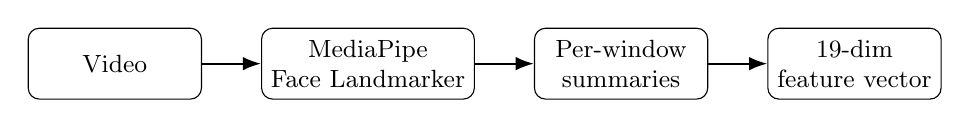
\begin{tikzpicture}[
      node distance=0.65cm and 0.75cm,
      box/.style={draw, rounded corners, align=center, minimum height=0.9cm, minimum width=2.2cm, font=\small},
      arr/.style={-Latex, thick}
    ]
    \node[box] (vid)  {Video};
    \node[box, right=of vid] (land) {MediaPipe\\Face Landmarker};
    \node[box, right=of land] (win)  {Per-window\\summaries};
    \node[box, right=of win]  (feat) {19-dim\\feature vector};
    \draw[arr] (vid)  -- (land);
    \draw[arr] (land) -- (win);
    \draw[arr] (win)  -- (feat);
  \end{tikzpicture}
  \end{center}
\end{frame}

% ---------------------------------------------------------------------------
% Slide 5 --- Model family (tightened to 3 bullets)
% ---------------------------------------------------------------------------
\begin{frame}
  \frametitle{Model family: tabular baselines vs.\ sequence model}
  \begin{itemize}
    \item \textbf{Classical:} Logistic Reg.\ / RF / XGBoost on per-window feature vectors.
    \item \textbf{Tabular NN:} MLP ($128\!\to\!64\!\to\!32$), FT-Transformer.
    \item \textbf{Sequence model (ours):} Bidirectional Mamba-1 via \texttt{mamba-ssm} fused CUDA kernel; $d_\text{model}=64$, $n_\text{blocks}=2$, $d_\text{state}=16$.
  \end{itemize}
\end{frame}

% ---------------------------------------------------------------------------
% Slide 6 --- Mamba block diagram
% ---------------------------------------------------------------------------
\begin{frame}
  \frametitle{Inside one Mamba block}
  \IfFileExists{../figures/mamba_block_diagram.png}{%
    \begin{center}
      \includegraphics[width=0.78\textwidth]{../figures/mamba_block_diagram.png}
    \end{center}
  }{%
    \begin{center}
    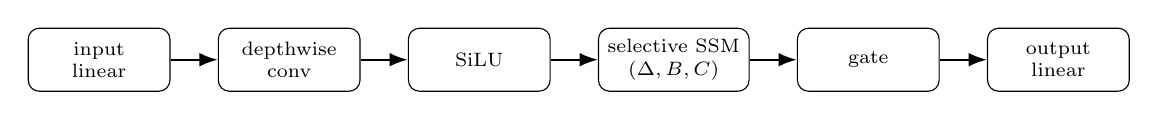
\begin{tikzpicture}[
        node distance=0.45cm and 0.6cm,
        box/.style={draw, rounded corners, align=center, minimum height=0.8cm, minimum width=1.8cm, font=\scriptsize},
        arr/.style={-Latex, thick}
      ]
      \node[box] (in)    {input\\linear};
      \node[box, right=of in]    (conv) {depthwise\\conv};
      \node[box, right=of conv]  (silu) {SiLU};
      \node[box, right=of silu]  (ssm)  {selective SSM\\($\Delta,B,C$)};
      \node[box, right=of ssm]   (gate) {gate};
      \node[box, right=of gate]  (out)  {output\\linear};
      \draw[arr] (in)   -- (conv);
      \draw[arr] (conv) -- (silu);
      \draw[arr] (silu) -- (ssm);
      \draw[arr] (ssm)  -- (gate);
      \draw[arr] (gate) -- (out);
    \end{tikzpicture}
    \end{center}
  }
  \vspace{0.3em}
  \small Bidirectional: forward and reversed Mamba layers are summed inside each residual block.
\end{frame}

% ---------------------------------------------------------------------------
% Slide 7 --- Cross-validation protocol (simplified)
% ---------------------------------------------------------------------------
\begin{frame}
  \frametitle{Cross-validation: 5-fold StratifiedGroupKFold by subject}
  \begin{itemize}
    \item Group key: \texttt{video\_id} (subject); 5 folds $\times$ 4 held-out subjects each.
    \item Leave-subjects-out: no subject appears in both train and validation within a fold.
    \item Metrics: per-window macro-F1 (primary); per-chunk majority-vote macro-F1 (secondary).
    \item Feature means/stds and class weights computed on the training fold only.
  \end{itemize}
\end{frame}

% ---------------------------------------------------------------------------
% Slide 8 --- Main result: at-a-glance
% ---------------------------------------------------------------------------
\begin{frame}
  \frametitle{Main result --- at-a-glance}
  \begin{itemize}[<+->]
    \item Mamba achieves window macro-F1 $= \mathbf{0.630 \pm 0.098}$ at the $\sigma = 0.1$ reference regime.
    \item Best tabular baseline (logreg) lands at $0.492$: a $\mathbf{+0.138}$ window-F1 lead for the sequence model.
  \end{itemize}
\end{frame}

% ---------------------------------------------------------------------------
% Slide 9 --- Main result: full table
% ---------------------------------------------------------------------------
\begin{frame}
  \frametitle{Main result --- full table}
  \centering
  \footnotesize
  \begin{tabular}{@{}lcc@{}}
    \toprule
    Model & Window macro-F1 & Chunk macro-F1 \\
    \midrule
    logreg            & $0.492 \pm 0.035$ & $\mathbf{0.685}$ \\
    rf                & $0.389 \pm 0.024$ & $0.430$ \\
    xgb               & $0.408 \pm 0.035$ & $0.440$ \\
    mlp               & $0.455 \pm 0.021$ & $0.526$ \\
    ftt               & $0.439 \pm 0.023$ & $0.452$ \\
    \textbf{Mamba-1 (ours)} & $\mathbf{0.630 \pm 0.098}$ & $0.652$ \\
    \bottomrule
  \end{tabular}

  \vspace{0.5em}
  {\footnotesize Fold-mean $\pm$ std at the $\sigma=0.1$ reference regime. Caveat: logreg narrowly wins chunk-F1 ($0.685$ vs $0.652$) because chunk-consistent per-window summaries benefit majority-vote aggregation.}
\end{frame}

% ---------------------------------------------------------------------------
% Slide 10 --- Robustness curve
% ---------------------------------------------------------------------------
\begin{frame}
  \frametitle{Robustness: paired-noise train-and-eval regime}
  \begin{center}
  \IfFileExists{../figures/fig3_robustness_curve.png}{%
    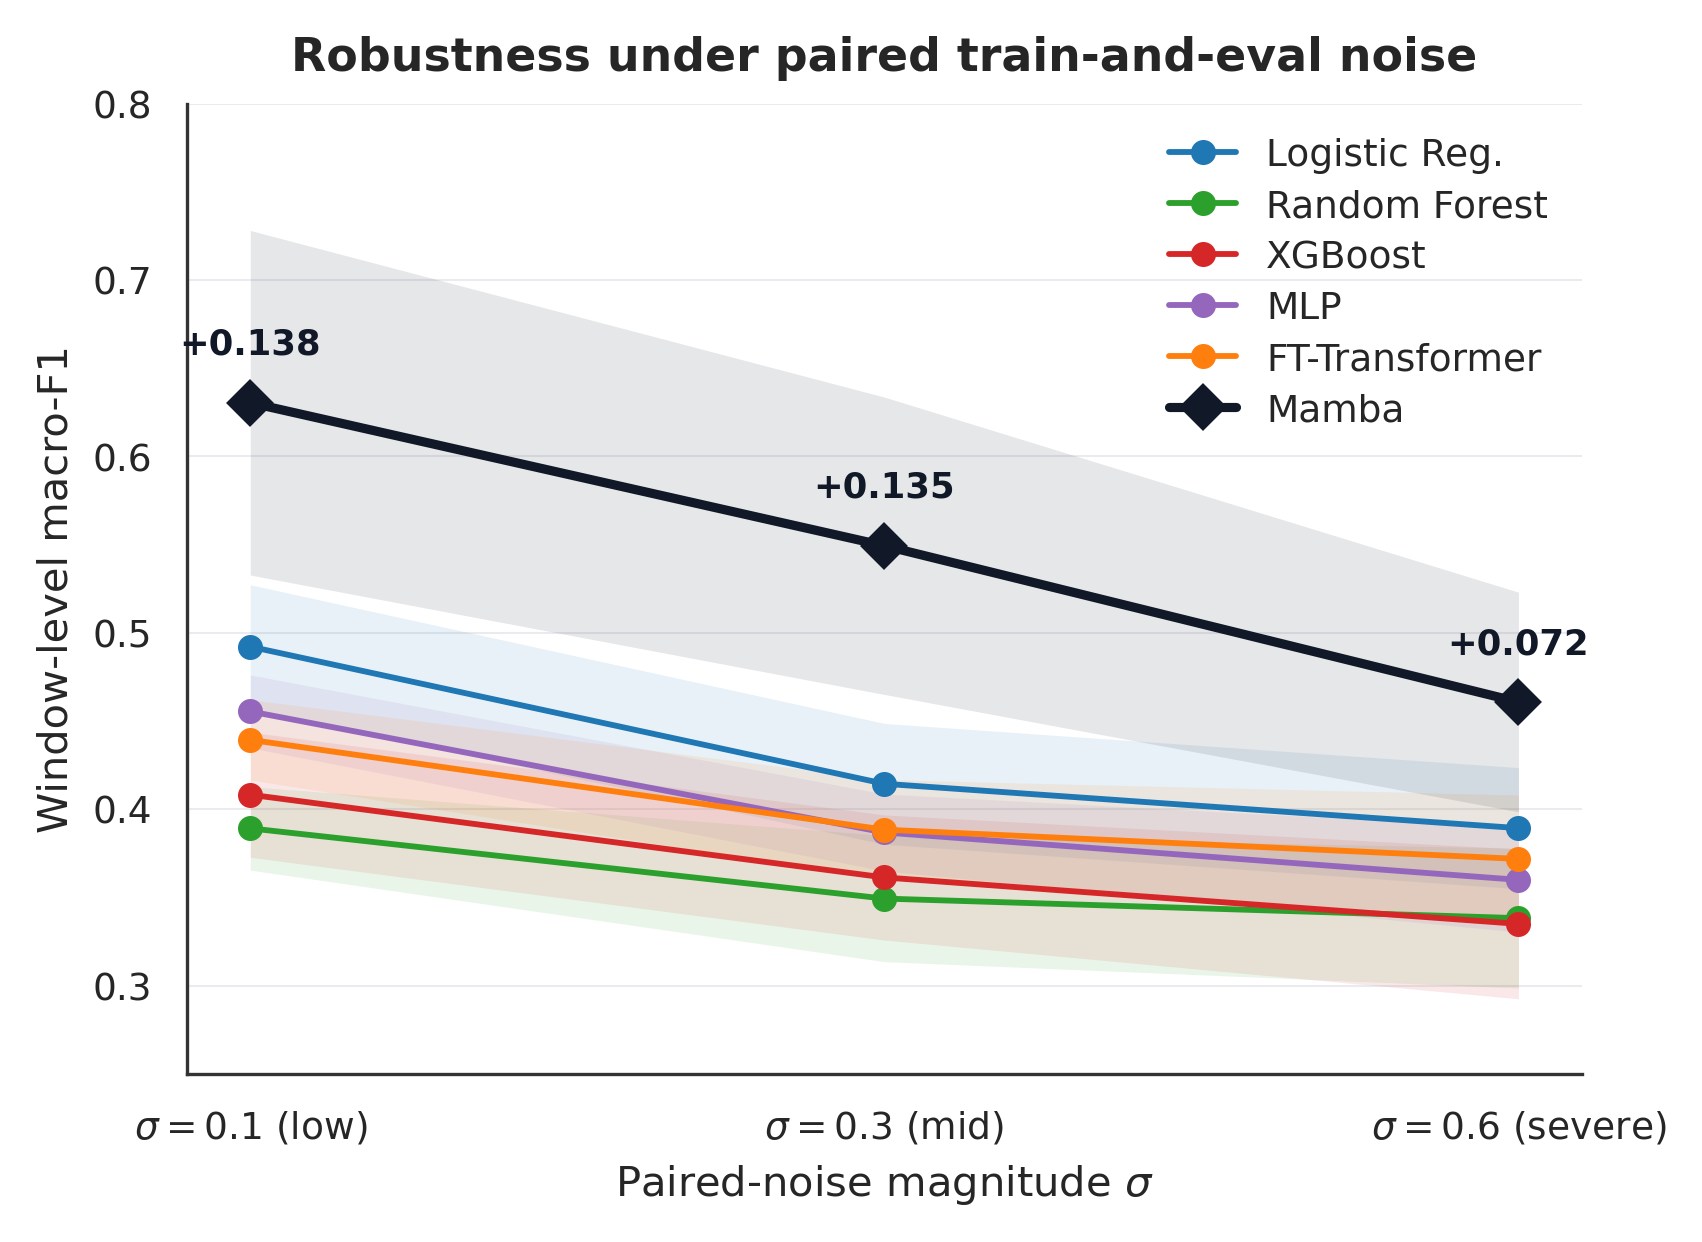
\includegraphics[width=0.62\textwidth]{../figures/fig3_robustness_curve.png}
  }{(figure pending)}
  \end{center}
  \footnotesize
  Per-window macro-F1 under a paired-noise train-and-eval regime at
  $\sigma \in \{0.1,\,0.3,\,0.6\}$. Mamba retains its absolute lead across all magnitudes;
  the gap narrows at $\sigma=0.6$ as all models converge toward chance under severe noise.
\end{frame}

% ---------------------------------------------------------------------------
% Slide 11 --- Confusion-matrix / per-class
% ---------------------------------------------------------------------------
\begin{frame}
  \frametitle{Per-class behavior: medium is the hardest class}
  \begin{center}
  \IfFileExists{../figures/fig2_confusion_matrices_low.png}{%
    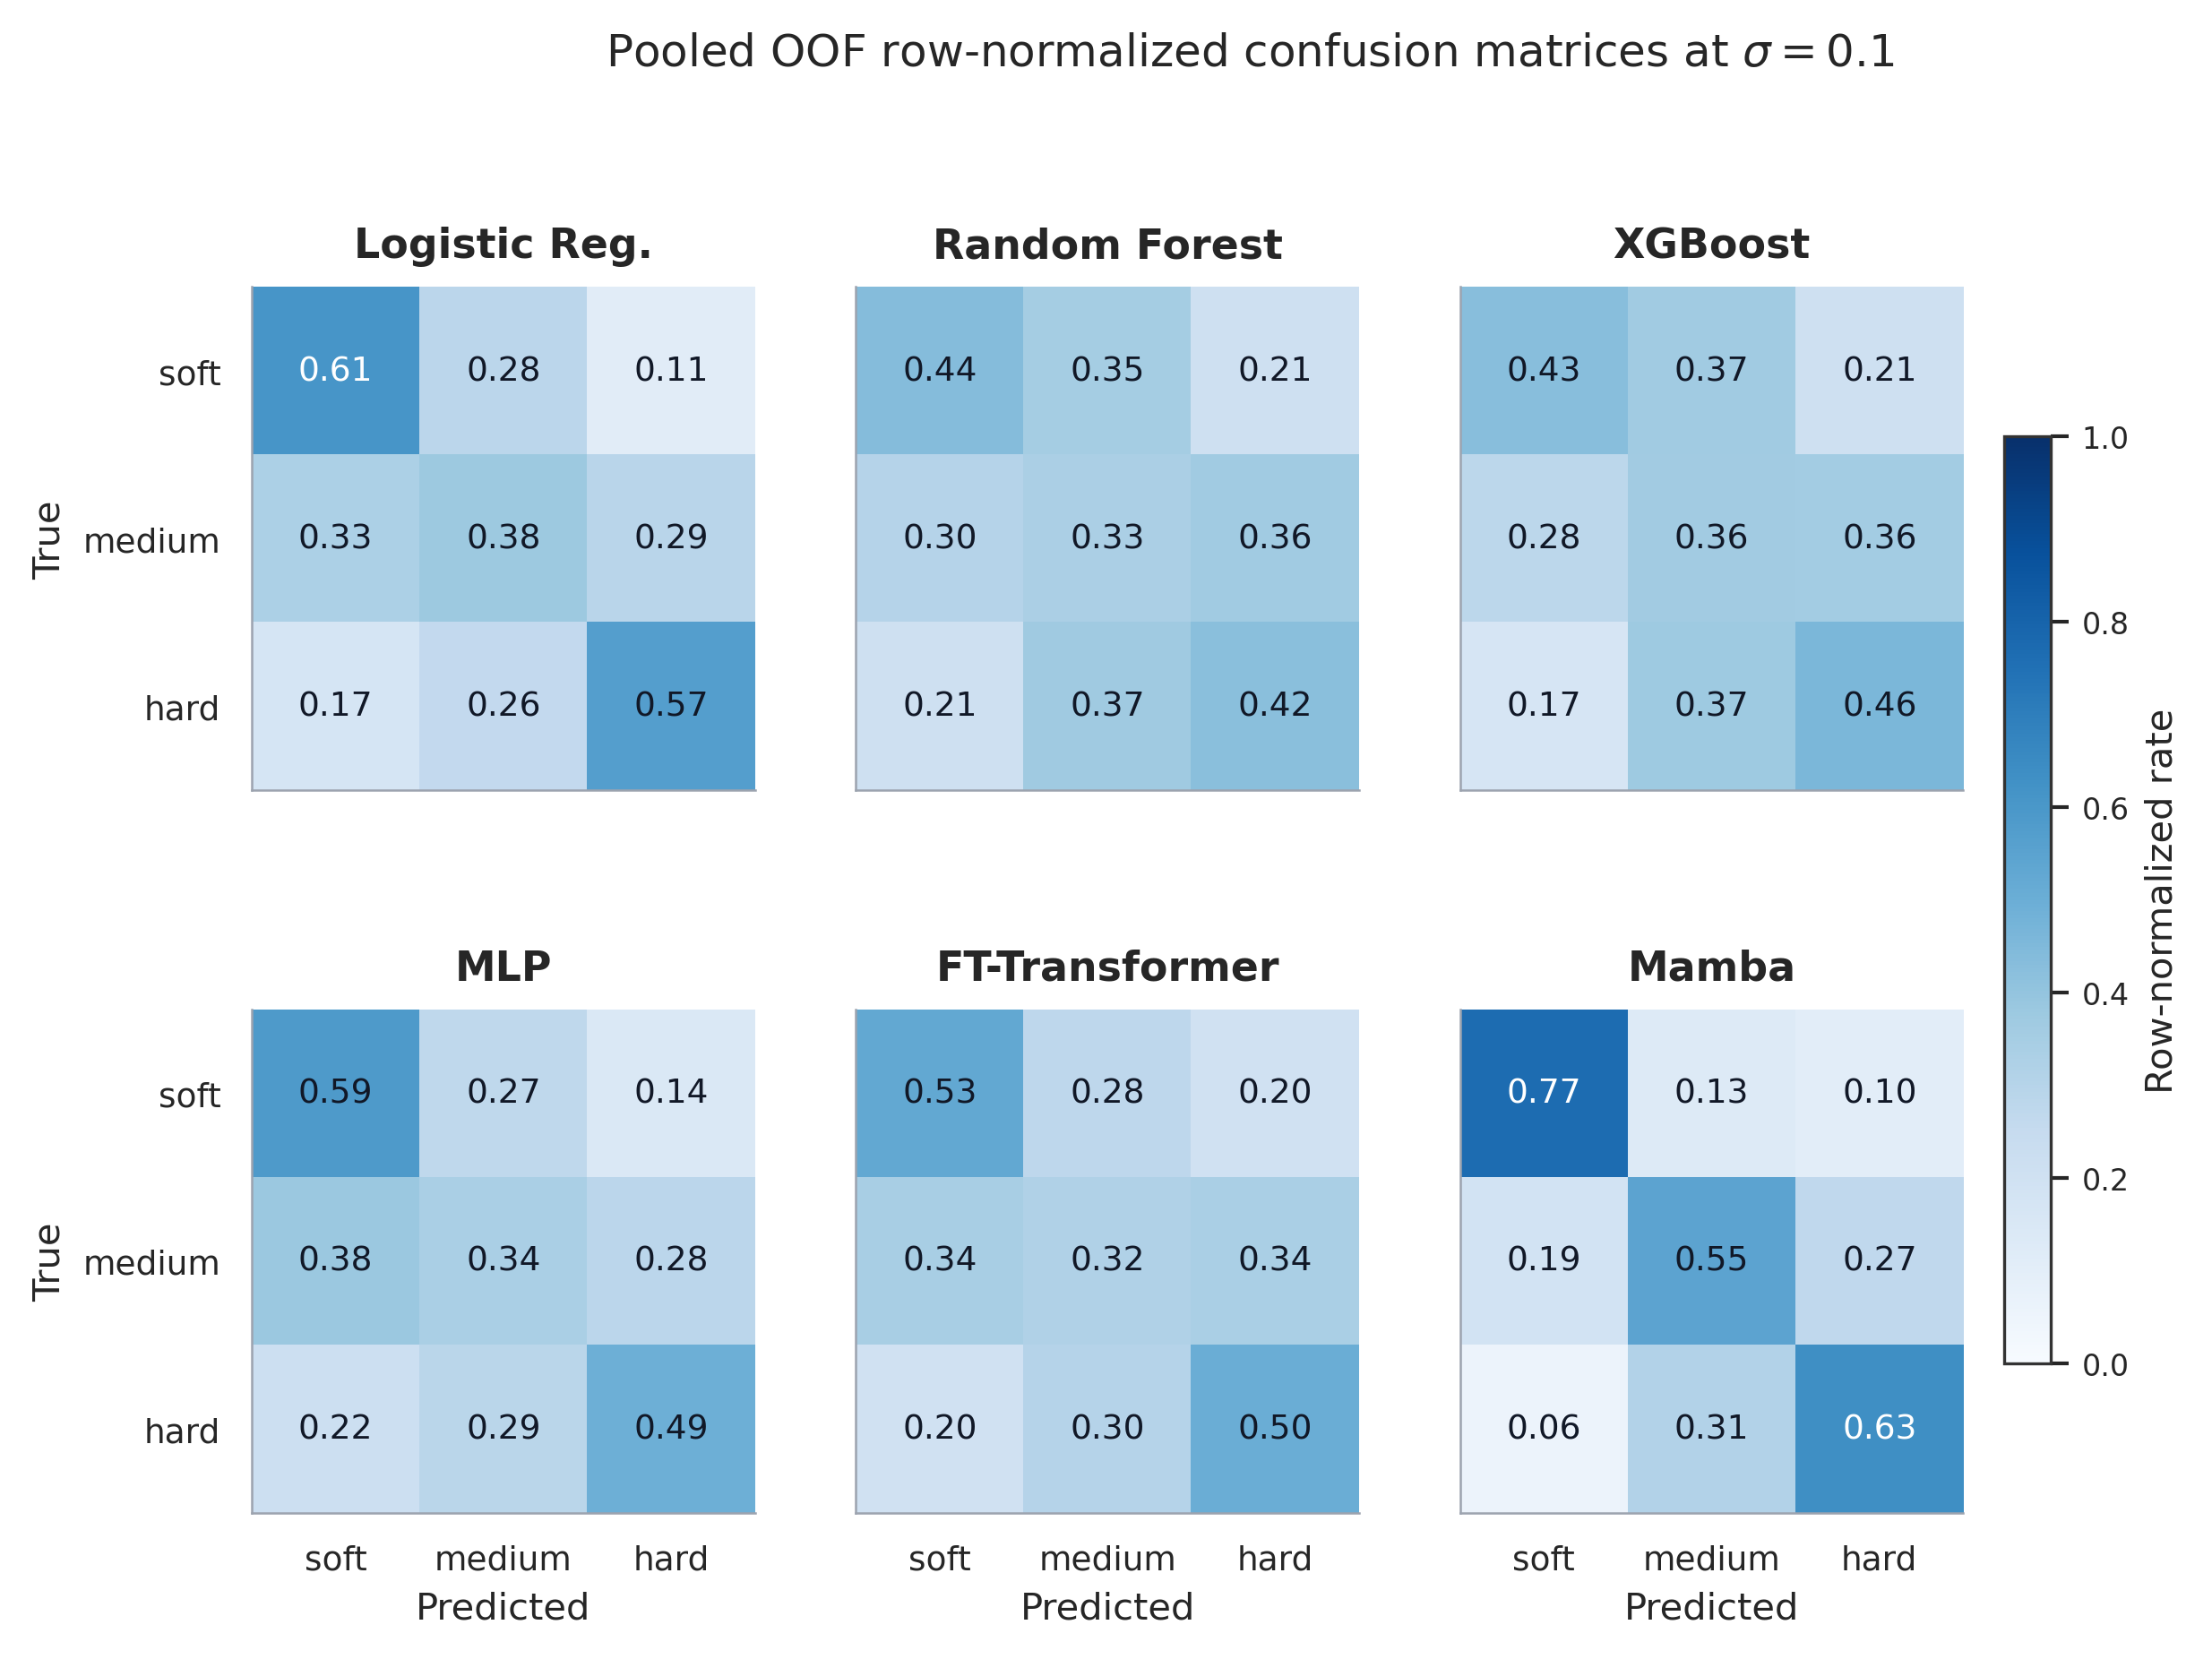
\includegraphics[width=0.70\textwidth]{../figures/fig2_confusion_matrices_low.png}
  }{(figure pending)}
  \end{center}
  \footnotesize
  Medium texture is the hardest class (Mamba per-class F1 $= 0.54$ vs soft $0.74$, hard $0.61$); most errors are between adjacent ordinal classes.
\end{frame}

% ---------------------------------------------------------------------------
% Slide 12 --- Ablation (matched-size)
% ---------------------------------------------------------------------------
\begin{frame}
  \frametitle{Ablation: Mamba-3 (hybrid) vs.\ Mamba-1 (matched-size baseline)}
  \begin{itemize}
    \item Mamba-3 (hybrid) wins by $+0.023$ window macro-F1 and $+0.046$ chunk macro-F1.
    \item Wall-clock cost $\approx 143\times$ the fused kernel (implementation-driven, not algorithmic).
  \end{itemize}

  \vspace{0.4em}
  \centering
  \footnotesize
  \begin{tabular}{@{}lcc@{}}
    \toprule
    Variant & Window macro-F1 & Chunk macro-F1 \\
    \midrule
    Mamba-1 (matched-size baseline)   & $0.373 \pm 0.036$ & $0.446$ \\
    Mamba-3 (matched-size hybrid)     & $0.396 \pm 0.026$ & $0.492$ \\
    $\Delta$                          & $+0.023$          & $+0.046$ \\
    \bottomrule
  \end{tabular}

  \vspace{0.3em}
  {\tiny Matched-size config: $d_\text{model}=32$, $n_\text{blocks}=1$, $d_\text{state}=8$, 30 epochs --- not comparable to the main Mamba result on Slide 9.}
\end{frame}

% ---------------------------------------------------------------------------
% Slide 13 --- Feature importance
% ---------------------------------------------------------------------------
\begin{frame}
  \frametitle{Feature importance: what the tabular models agree on}
  \begin{center}
  \IfFileExists{../figures/fig4_feature_importance_top10.png}{%
    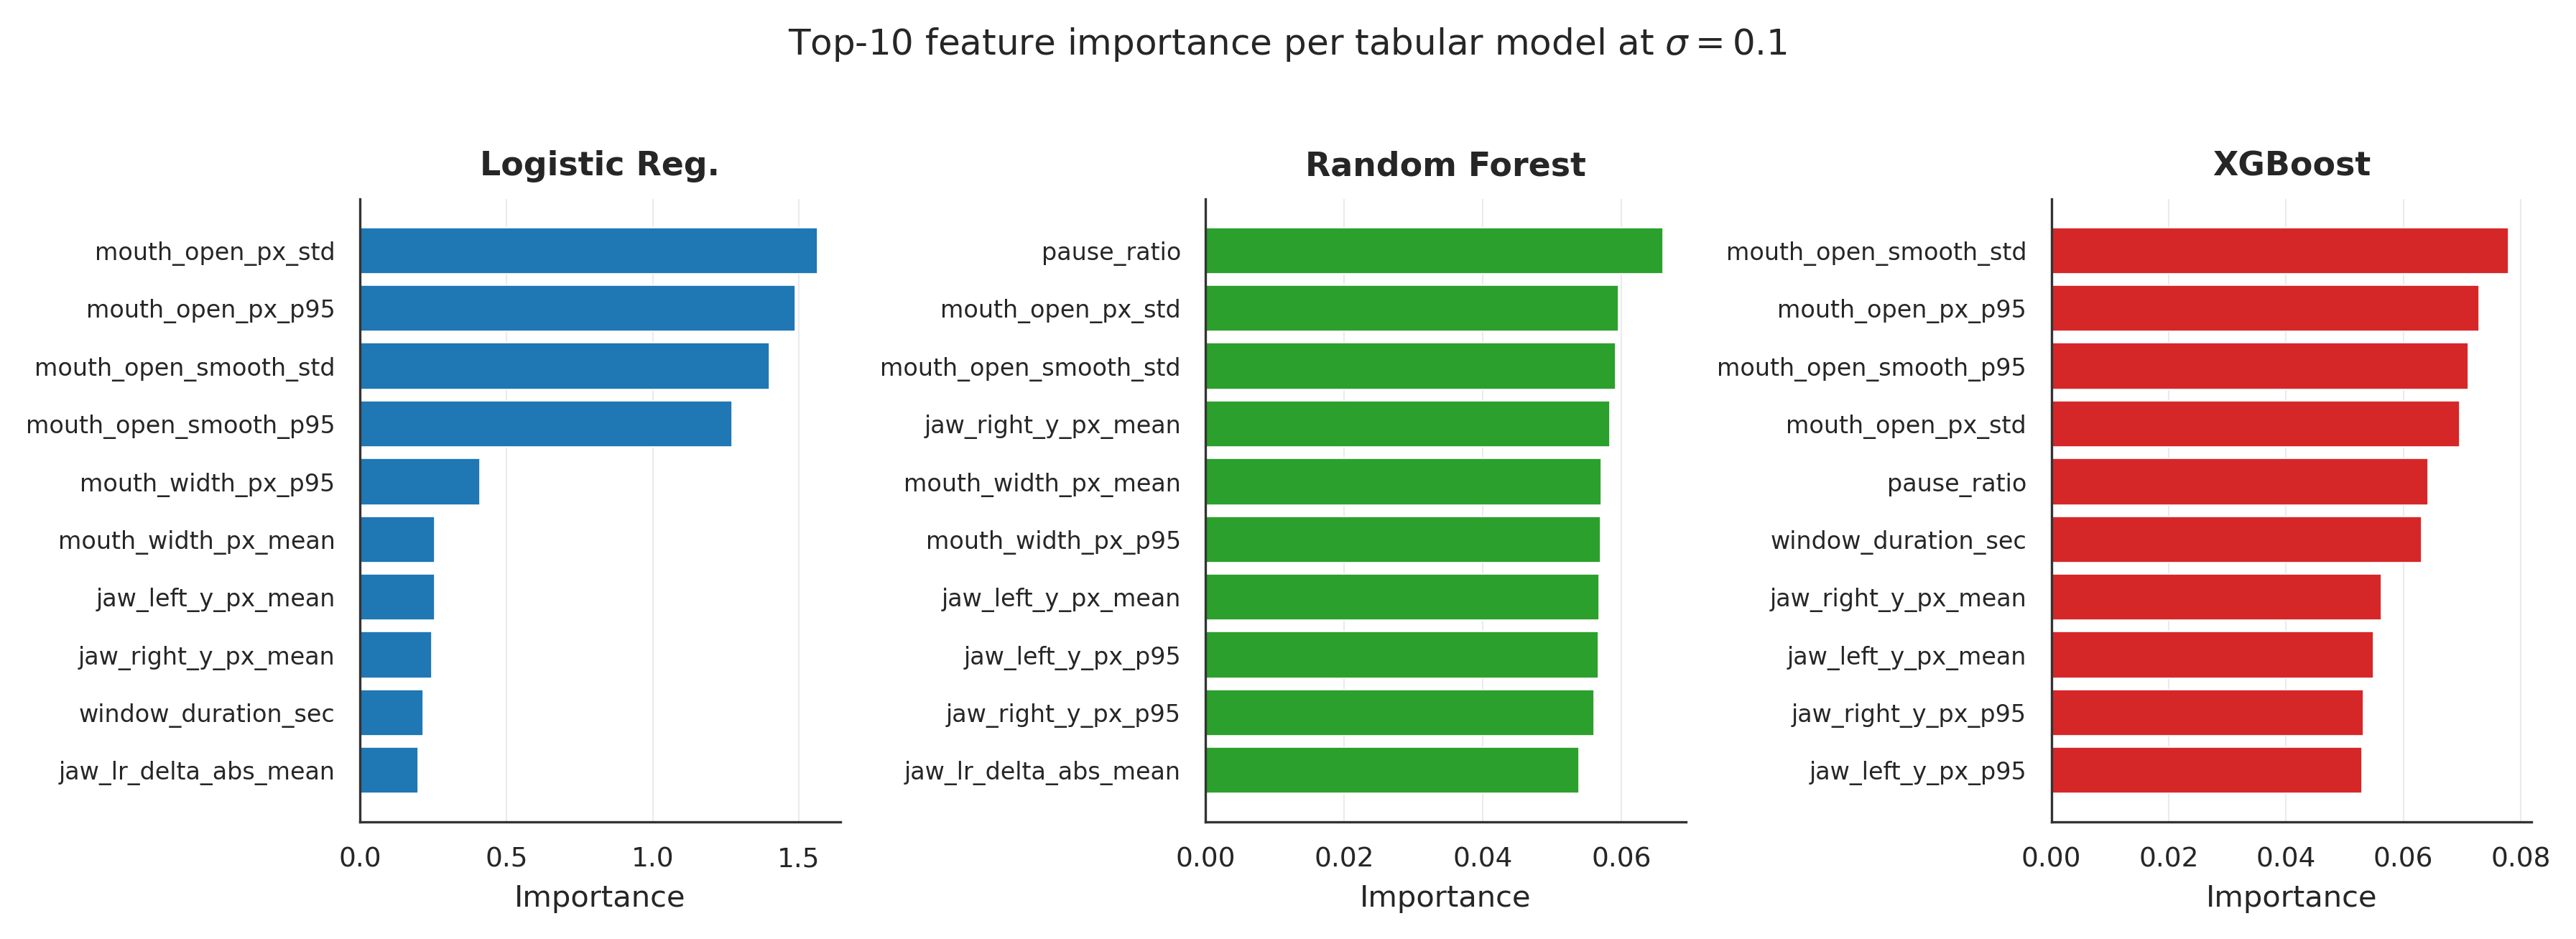
\includegraphics[width=0.72\textwidth]{../figures/fig4_feature_importance_top10.png}
  }{(figure pending)}
  \end{center}
  \footnotesize
  Mouth-open variability (std, p95) is the dominant signal across all three tabular models;
  pause\_ratio is additionally highly ranked by rf and xgb. Harder foods elicit larger-amplitude,
  more variable chewing motion with fewer low-activity intervals.
\end{frame}

% ---------------------------------------------------------------------------
% Slide 14 --- Limitations and future work
% ---------------------------------------------------------------------------
\begin{frame}
  \frametitle{Limitations and next steps}
  \begin{itemize}
    \item Cohort size: 20 subjects, 4 per held-out fold --- fold-mean numbers carry real uncertainty.
    \item Per-fold Mamba window-F1 std $= 0.098$, largest among models: subject-level instability.
    \item Ablation trained at 30 epochs (tiny config) vs 80 epochs (main) --- budget-matched comparison is future work.
    \item Single seed per fold; multi-seed averaging would harden the ranking.
    \item Follow-ups: larger cohort; GRU / TCN / small-Transformer sequence baselines;
          fused CUDA kernel for Mamba-3 upgrades; finer-grained (frame-level) modeling; multi-modal fusion.
  \end{itemize}
\end{frame}

% ---------------------------------------------------------------------------
% Slide 15 --- Conclusion and Q&A
% ---------------------------------------------------------------------------
\begin{frame}
  \frametitle{Conclusion and Q\&A}
  \begin{itemize}
    \item Selective state-space models are a credible inductive-bias choice for
          chewing-video texture classification.
    \item Headline: $+0.138$ window-F1 over the strongest tabular baseline at $\sigma = 0.1$;
          preserves a $+0.072$ lead even at $\sigma = 0.6$.
    \item Open: specifically \emph{selective} SSMs vs.\ other sequence families;
          scaling to larger cohorts; fused kernels for Mamba-3-style refinements.
  \end{itemize}
  \vspace{1.0em}
  \begin{center}
    \Large Questions?
  \end{center}
\end{frame}

\end{document}
